\documentclass{article}

% Language setting
% Replace `english' with e.g. `spanish' to change the document language
\usepackage[english]{babel}

% Set page size and margins
% Replace `letterpaper' with`a4paper' for UK/EU standard size
\usepackage[letterpaper,top=2cm,bottom=2cm,left=3cm,right=3cm,marginparwidth=1.75cm]{geometry}


% Useful packages
\usepackage{amsmath}
\usepackage{graphicx}
\usepackage[colorlinks=true, allcolors=blue]{hyperref}
\usepackage{float}
\usepackage{caption}
\usepackage{subcaption}
\usepackage[demo]{graphicx}
%Path
\graphicspath{{figures/}}

\title{Modelling Nisq Computers}
\author{Kristian Wold}

\begin{document}
\maketitle

\section{Introduction}

\section{Choi Form}

\subsection{Comparing Gradient Descent with Adam Optimizer}

\subsection{Overparameterized Choi Form}

\section{Kraus Form}

\subsection{Fitting Kraus Form with Prior Unitary}

\subsection{Fitting Low Rank Kraus Maps to High Rank Kraus Maps}

\subsection{Sparse Input}


\section{Real Hardware}

\section{Interesting Quantum Maps}


\begin{figure}[htbp]
\begin{subfigure}[t]{0.3\textwidth}
    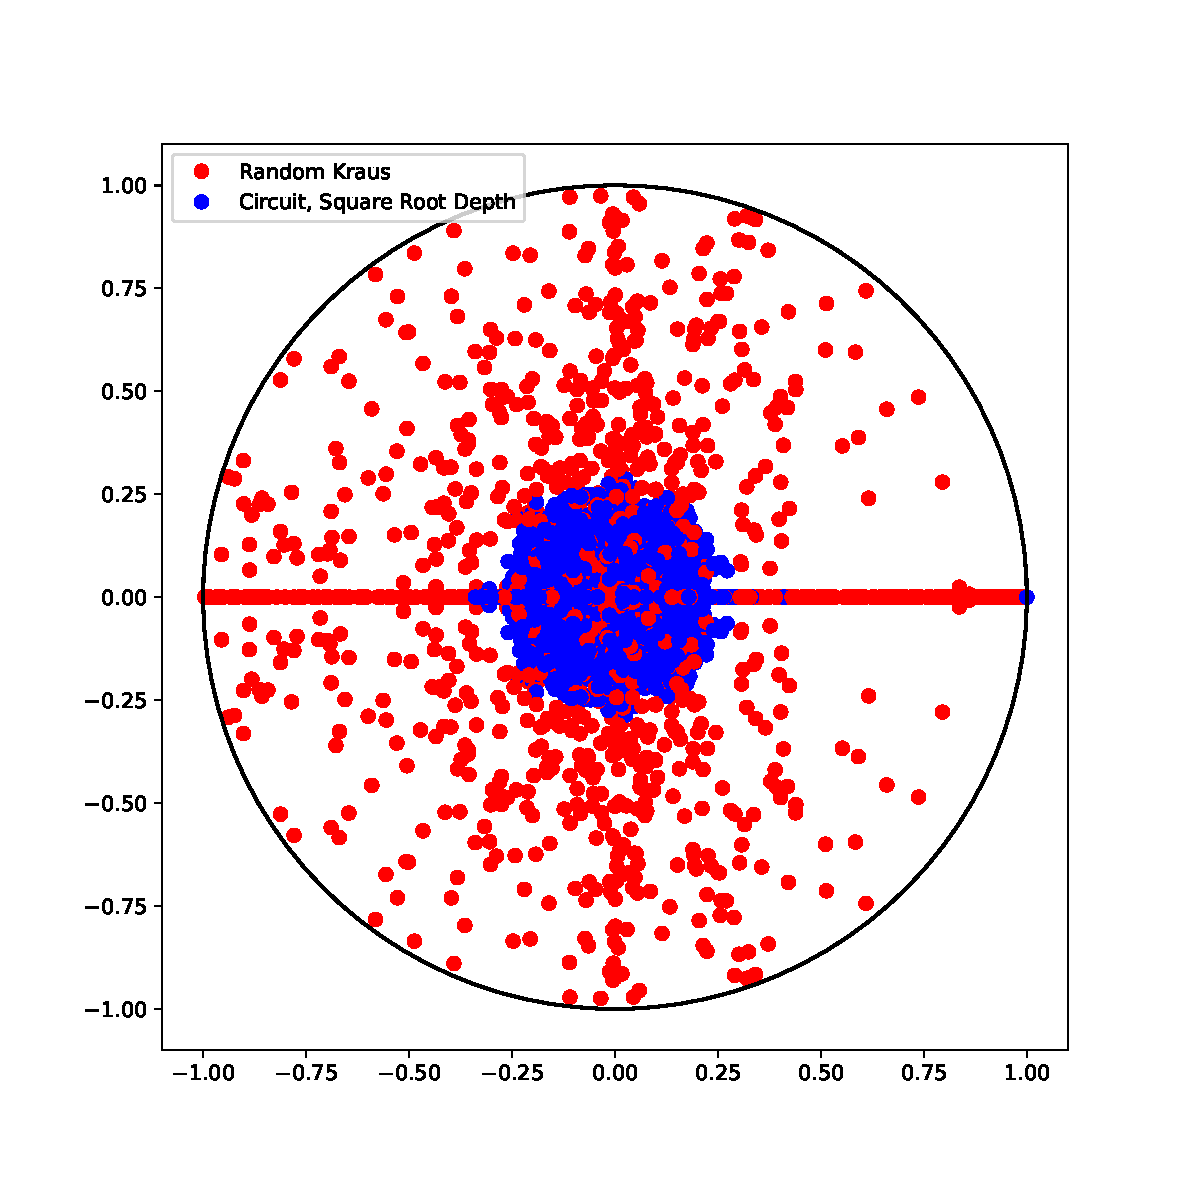
\includegraphics[width=\linewidth]{../figures/twoQubit_squareRootDepth}
\caption{Two Qubits}
\label{fig:figure14_1}
\end{subfigure}\hfill
\begin{subfigure}[t]{0.3\textwidth}
  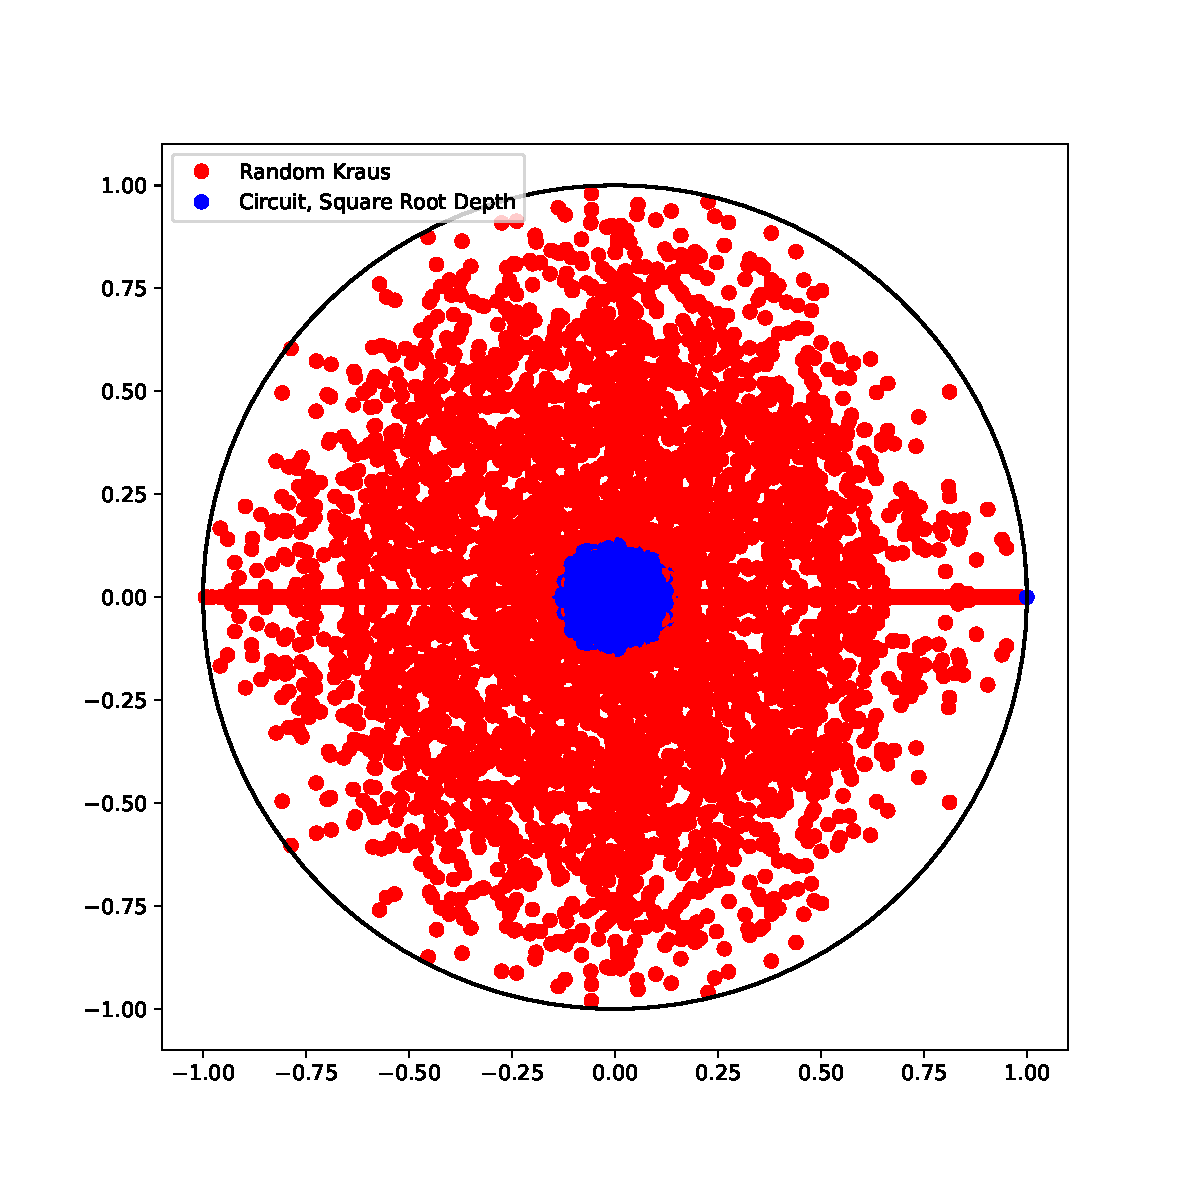
\includegraphics[width=\linewidth]{../figures/threeQubit_squareRootDepth}
\caption{Three Qubits}
\label{fig:figure14_2}
\end{subfigure}\hfill
\begin{subfigure}[t]{0.3\textwidth}
    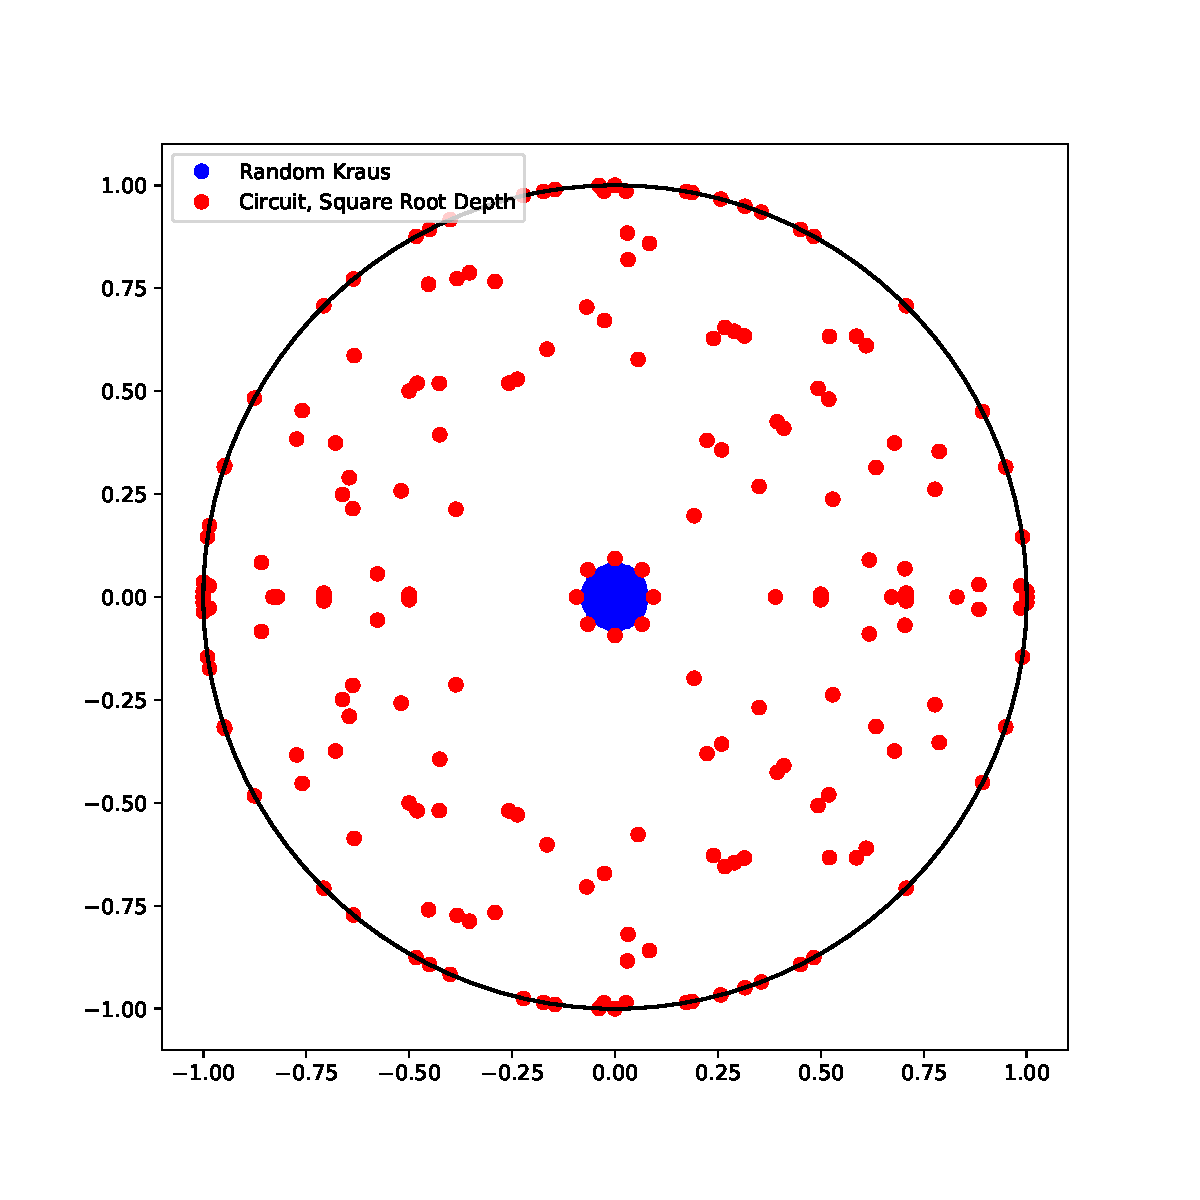
\includegraphics[width=\linewidth]{../figures/fourQubit_squareRootDepth}
\caption{Four Qubits}
\label{fig:figure14_3}
\end{subfigure}

\begin{subfigure}[t]{0.3\textwidth}
    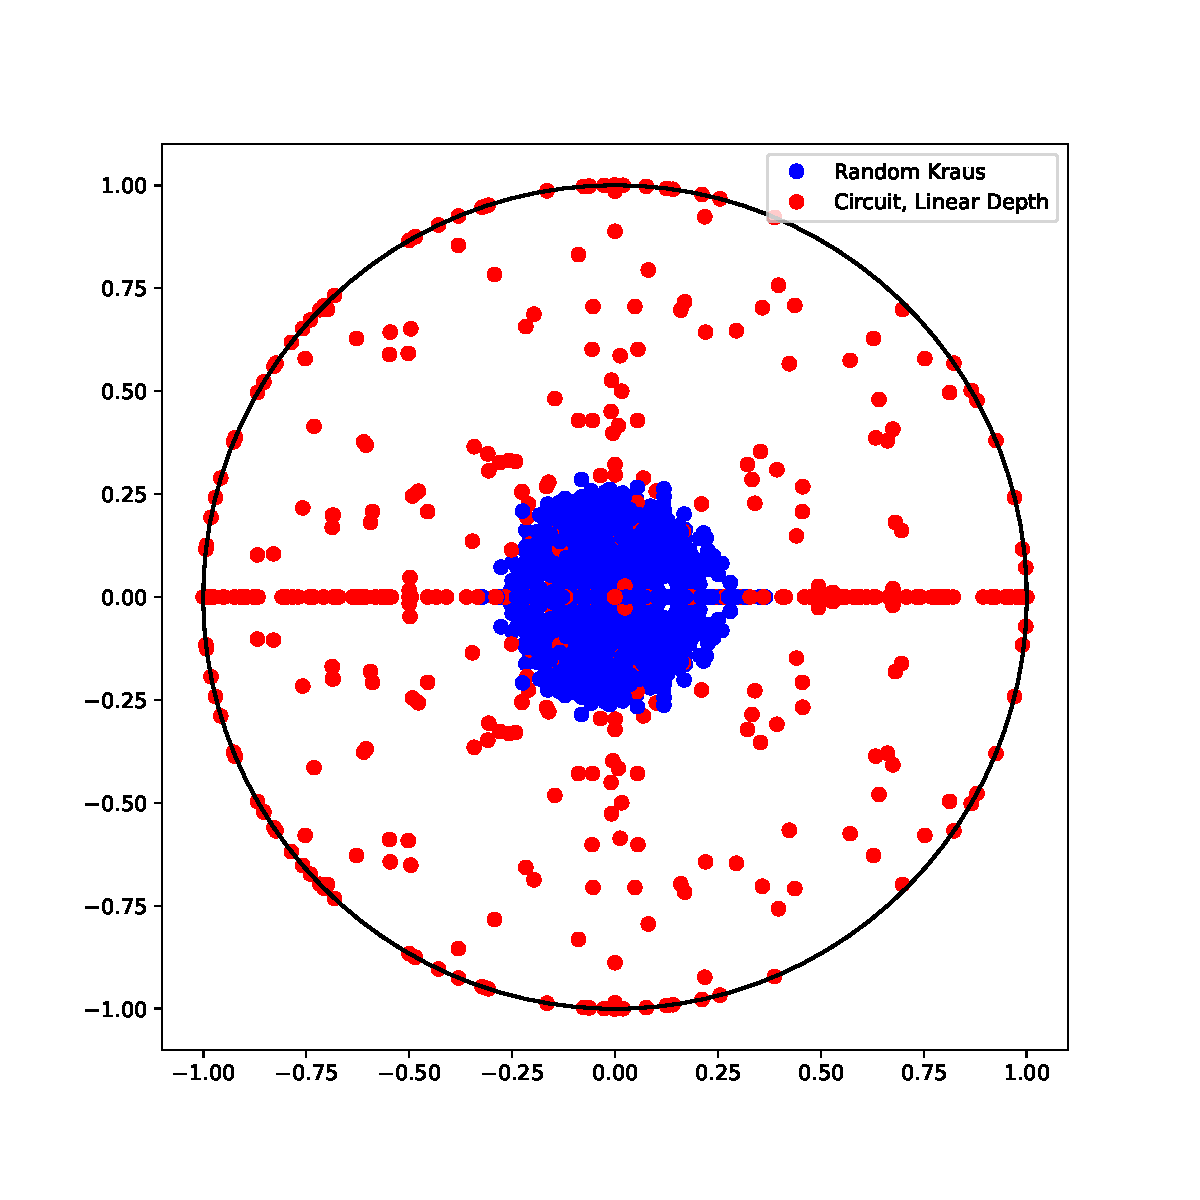
\includegraphics[width=\linewidth]{../figures/twoQubit_linearDepth}
\caption{Two Qubits}
\label{fig:figure14_4}
\end{subfigure}\hfill
\begin{subfigure}[t]{0.3\textwidth}
    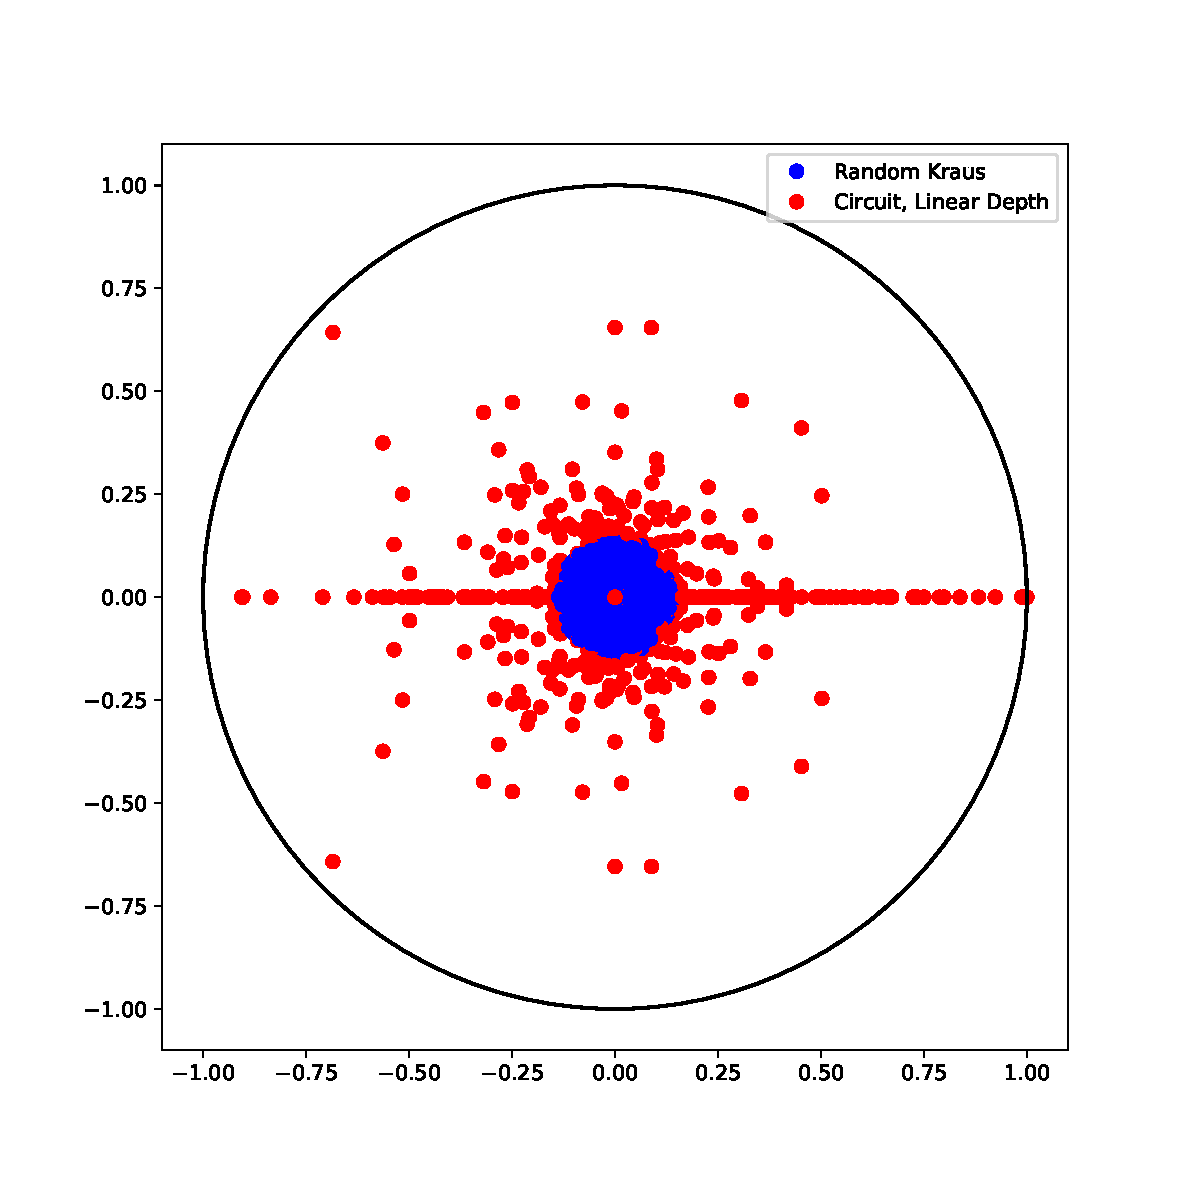
\includegraphics[width=\linewidth]{../figures/threeQubit_linearDepth}
\caption{Three Qubits}
\label{fig:figure14_5}
\end{subfigure}\hfill
\begin{subfigure}[t]{0.3\textwidth}
    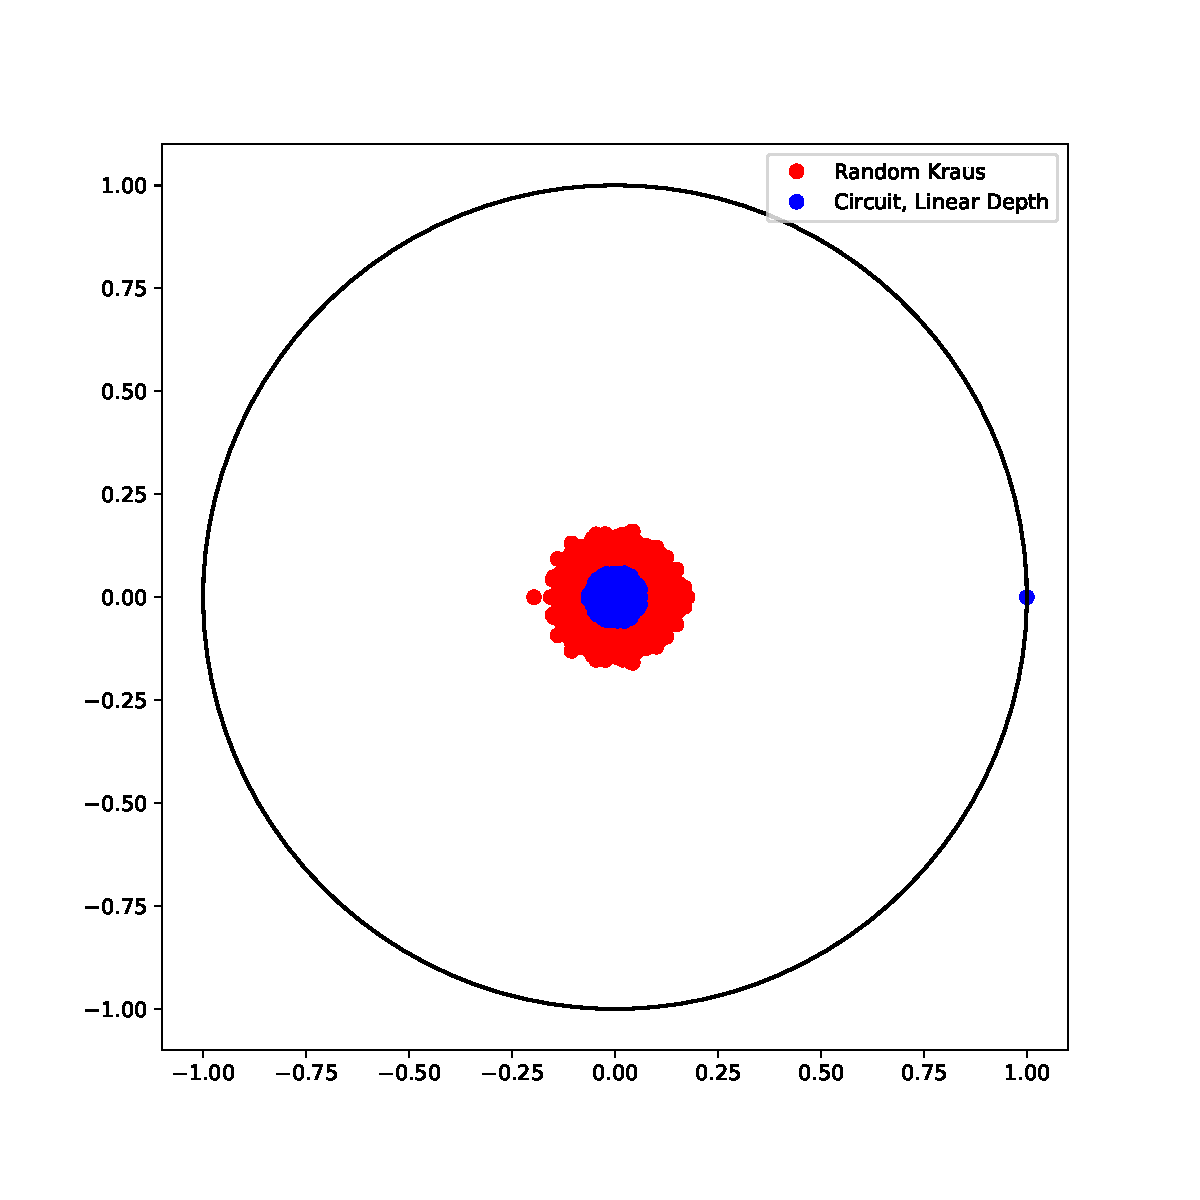
\includegraphics[width=\textwidth]{../figures/fourQubit_linearDepth}
\caption{Four Qubits}
\label{fig:figure14_6}
\end{subfigure}

\begin{subfigure}[t]{0.3\textwidth}
    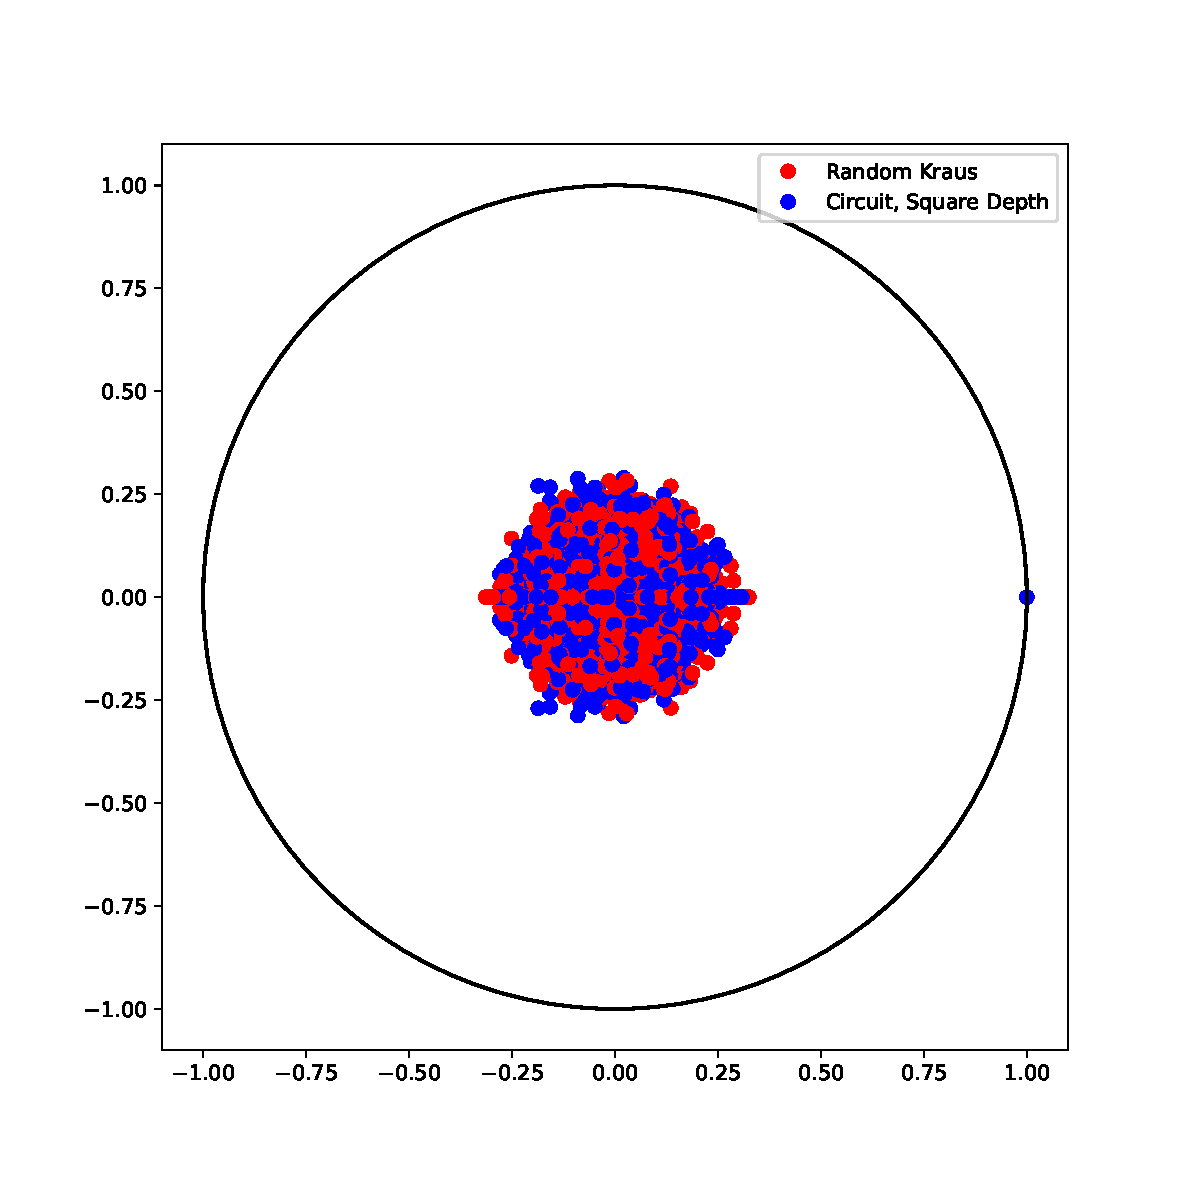
\includegraphics[width=\linewidth]{../figures/twoQubit_squareDepth}
\caption{Two Qubits}
\label{fig:figure14_7}
\end{subfigure}\hfill
\begin{subfigure}[t]{0.3\textwidth}
    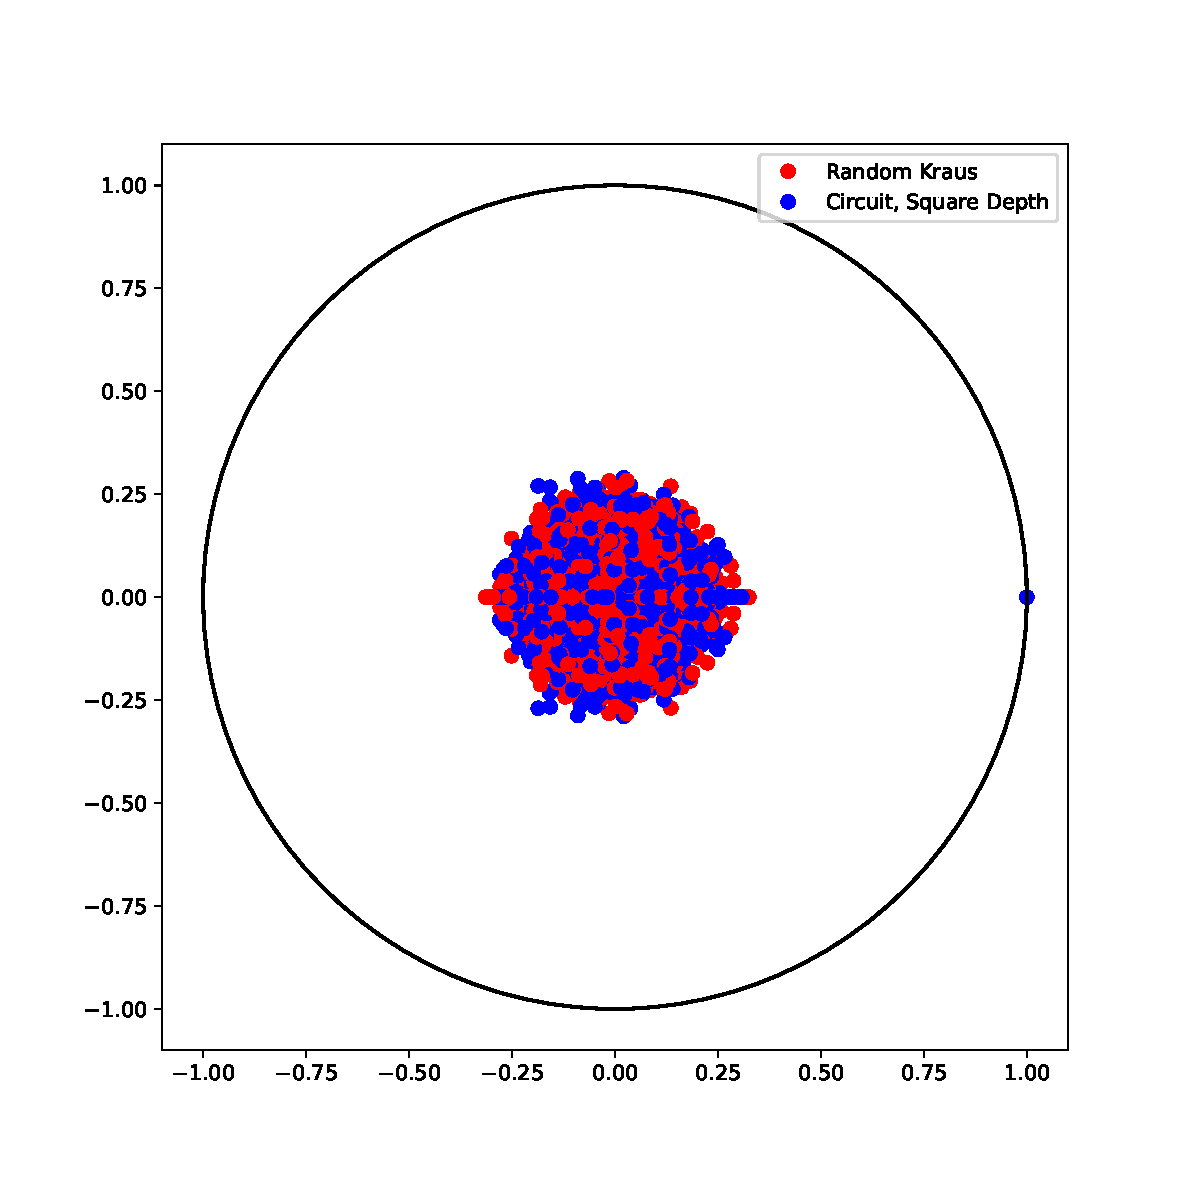
\includegraphics[width=\linewidth]{../figures/twoQubit_squareDepth}
\caption{Three Qubits}
\label{fig:figure14_8}
\end{subfigure}\hfill
\begin{subfigure}[t]{0.3\textwidth}
    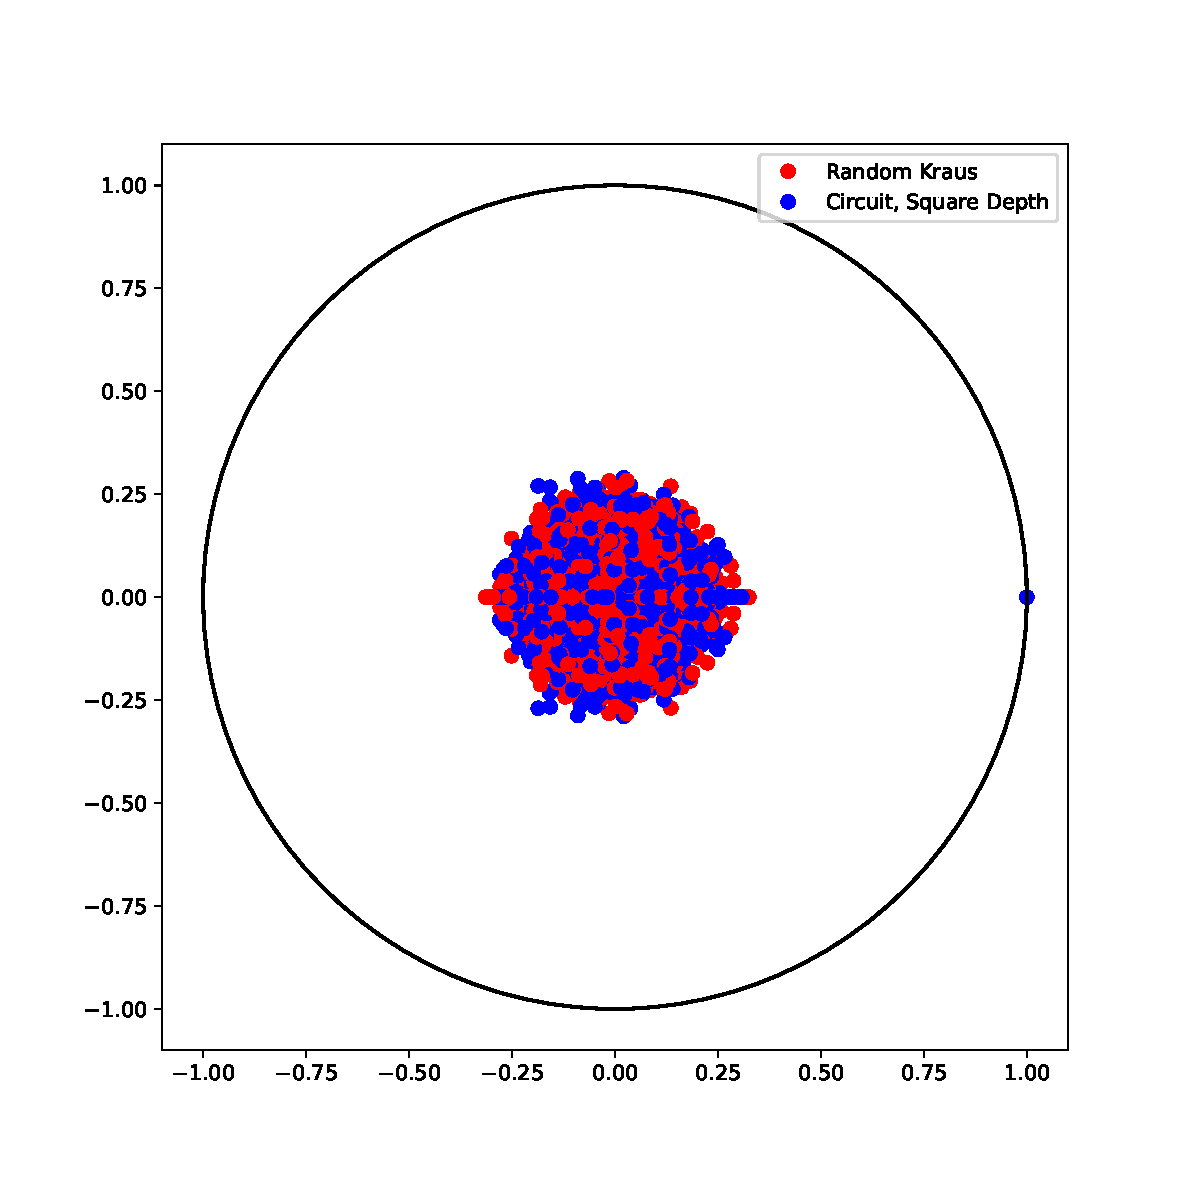
\includegraphics[width=\linewidth]{../figures/twoQubit_squareDepth}
\caption{Four Qubits}
\label{fig:figure14_9}
\end{subfigure}

\caption{3-point bending, elastic and plastic stress distribution, 
    shaft under torsion load and linearly distributed load.}
\label{figure14_99}
\end{figure}



\bibliographystyle{alpha}
\bibliography{sample}

\end{document}